\chapter{Fleet-Scale Analytics on the Log}
\label{chap:analytics}

Chapter~\ref{chap:design} produced a substrate: every observable event of
the fleet, durably ordered, attributed to node and agent, readable hot or
cold. This chapter presents the analyses that turn that substrate into
answers to the operator questions of \S\ref{sec:problem-scenario}. Each
section follows the same shape: the question, the algorithm, and the
argument for why it stays cheap at fleet scale.

\section{Live Topology Coupling: Scenario Graph and Cluster Graph}
\label{sec:analytics-topology}

The first question (Q1) is situational awareness: what is the swarm doing,
right now, and where. The system answers it with two live graphs, built
deliberately as \emph{two projections of the same event stream}.

The \emph{scenario graph} projects Path-B edges onto agent identity: nodes
are sessions (\texttt{role@scenario}), edges are stitched calls labeled
with tool, status, and latency, built incrementally in the browser from the
live bus: backlog first, then per-event frames
(\S\ref{sec:design-read}). LLM-observability tools already offer this view
(\S\ref{sec:bg-sota-llm}); here it is rendered live. The \emph{cluster graph} projects
the very same edges onto physical topology: hosts as nodes, aggregated
host-pair traffic as edges (counts, error counts, active agents per host),
computed by folding the hot store. Because every edge carries
\texttt{from\_host} and \texttt{to\_host} stamped at capture (R1), the
projection is a group-by, not an inference.

The coupling is completed by the scheduler's view of the machine: the
dashboard queries SLURM (\texttt{sinfo}) for the allocation and the
cluster's total/idle/busy/down states, draws idle-but-available nodes
alongside the active deployment, and uses only real node names throughout.
A node with no events is drawn grey, not omitted; at fleet scale,
silence is a signal (R4). Clicking through connects the layers: an agent
node opens that agent's conversation (the \texttt{role@scenario} join of
\S\ref{sec:design-mapping}); a host cell pivots to the per-node view. This
two-projection design (same events, agent layer and machine layer) is
the direct answer to the gap of \S\ref{sec:bg-sota-gap}.

\section{ChronoDoctor: Detection, Clustering, and Diagnosis}
\label{sec:analytics-doctor}

The second question (Q2) is not ``show me the errors'' but ``tell me what
is wrong'': at fleet scale, a per-event error feed is least readable
when it matters most. ChronoDoctor is a five-stage pipeline
(\emph{gather} $\to$ \emph{detect} $\to$ \emph{cluster} $\to$
\emph{diagnose} $\to$ \emph{remember}) that turns raw events into a
ranked list of explained incidents.

\paragraph{Gather and detect.} Gathering is the only I/O: interactions and
recoveries from the Path-A spool (hot, GIL-safe), stitched edges from the
Path-B hot store, with explicit bounds on sessions and scenarios scanned.
Detection is a set of pure, unit-tested functions over the gathered lists,
each emitting typed \emph{signals}: HTTP 4xx/5xx and explicit errors on
turns (429 classified separately as rate-limiting); latency outliers,
flagged relative to the \emph{per-model} median (an absolute threshold
would misclassify a slow model as an incident); retry storms (the same
prompt re-issued repeatedly within a session); failed inter-agent calls;
\emph{orphan calls} (a \texttt{start} with no \texttt{done}, the
signature of a hung or dropped delegation); slow edges relative to the
per-tool median; and recovery events. Orphan calls are always ranked
critical: the delegating agent is silently stalled, and no per-edge view
shows anything wrong.
Detection is a single pass: $O(n)$ in gathered events, with per-group
medians over small per-model and per-tool groups.

\paragraph{Clustering.} The insight that makes the view scale is that
fleet-wide failures are \emph{textually self-similar}. Each signal's
message is normalized, with identifiers, hex runs, and digit strings replaced
by placeholders (\texttt{peer ares-comp-12 timed out after 30001ms}
$\to$ \texttt{peer ares-comp-<n> timed out after <n>ms}), and the pair
(kind, normalized message) is hashed into a \emph{signature}, the
clustering key. Five hundred identical timeouts across the fleet collapse
into one incident with a count of 500; hosts, sessions, tools, models, and
scenarios are aggregated \emph{inside} the incident as its blast radius,
deliberately excluded from the key so that a fleet-wide failure stays one
card while its distribution stays visible. Severity escalates with count,
and incidents rank by (severity, count, hosts affected), worst first.

\paragraph{Diagnosis.} Each incident gets a diagnosis (root cause,
remediation, blast radius, confidence) from a deterministic,
first-match-wins rule engine keyed on signal kind and sample text: orphan
calls map to hung-peer causes, 429s to rate limiting, transport-layer
markers to network-fabric issues, token-overflow patterns to context
exhaustion, and so on, each with a calibrated confidence; a conservative
fallback catches the rest. The engine costs nothing per scan (R6). An
LLM-backed diagnoser can be enabled explicitly, and any failure of it falls
back to the heuristic: the deterministic path is the contract, the LLM
an enhancement.

\paragraph{Memory.} The final stage answers Q5. Every scan appends one line
per incident to a Markdown incident memory; when the recent section
exceeds a threshold, the oldest lines fold into a digest with running
counts; the file is \emph{self-compacting}, so it stays small across
arbitrarily many runs while retaining per-signature totals. On each scan,
current incidents are matched against remembered signatures, and a repeat
offender is badged \texttt{recurring $\times N$}. The memory is a plain
human-readable file: the operator can read, annotate, or delete it, and it
survives restarts by construction.

\section{Fleet Health at Scale}
\label{sec:analytics-fleet}

The fourth question (Q4) is population-level: which node is unlike the
others. The node-link rendering of \S\ref{sec:analytics-topology} answers
it only up to a dozen nodes; past that, it is spaghetti. The fleet view
therefore changes representation (a heatmap grid, one cell per node,
colored by health, worst first) and, more fundamentally, changes the
\emph{read complexity}.

Computing node health from raw events is $O(\text{events})$ per refresh,
untenable as history grows. The system instead maintains
\emph{rollups}: for each (host, minute) pair, a bucket aggregating that
minute's activity (event and error counts, latency sum/count/p95/max,
token and cost totals, distinct agents). An emitter recomputes and appends
full bucket snapshots to a dedicated rollup story; because each append is a
complete snapshot of its cell, the reader keeps the last value seen per key
and re-emission never double-counts: idempotence by
last-writer-wins, the same discipline as \S\ref{sec:design-write}. A
health query then folds only the buckets in the requested window:
$O(\text{nodes} \times \text{buckets})$, independent of event volume (R4).
Per-node health folds by explicit rules: sums for counts, a ratio for
error rate, and the \emph{maximum} of per-minute p95s as the
window's p95 estimate (an upper-biased estimate that avoids retaining raw
samples). Thresholds then classify each node ok/warn/critical. Nodes in
the allocation that produced nothing are injected as empty rows, and every
row is tagged with its live SLURM state, so the grid always shows the
whole population. The emitter is optional. Absent rollups, the API falls
back to folding raw events on demand, which is correct at small scale and
keeps the tab from ever being empty.

\section{Cross-Host Critical-Path Tracing}
\label{sec:analytics-tracing}

The third question (Q3), why this scenario is slow, is the classical
tracing question of \S\ref{sec:bg-tracing}, posed across hosts. The tracer
reconstructs call trees from stitched Path-B edges in two steps.

\paragraph{Tree reconstruction.} Each stitched edge is a span: an interval
on the timeline from \texttt{start} to \texttt{done}, with endpoints,
tool, status, and latency. Parentage is resolved by a two-tier rule
mirroring \S\ref{sec:design-mapping}: if a span carries an explicit
\texttt{parent\_correlation\_id}, that is its parent, the
Dapper-style ground truth. Otherwise the parent is \emph{inferred}: the
span whose callee session matches this span's caller session and whose
interval encloses this span's (the tightest such enclosure winning),
on the Mystery-Machine premise that a delegation issued by agent $B$ while
$B$ was servicing a call must be causally nested within it. Spans with no
parent are roots; each root yields one trace, with depth assigned by tree
walk.

\paragraph{Critical path and bottleneck.} Within a trace, end-to-end
latency is attributed by the analysis of \S\ref{sec:bg-critpath}: the
critical path is walked from the root by descending into the slowest
child at each level, and each hop on the path is charged its
\emph{self-time} (its latency minus its slowest child's), so that
time spent waiting on a child is charged to the child, not double-counted
in the parent. The hop with maximal self-time is named the
\emph{bottleneck}, with its hosts and tool: not ``the scenario is slow''
but ``the \texttt{writer}$\to$\texttt{reviewer} hop on
\texttt{ares-comp-07}, 4.2\,s of self-time.'' Because hosts ride on every
span, the pivot to Q4 is immediate: if the bottleneck's node also glows in
the fleet heatmap, the cross-layer diagnosis (fleet symptom, physical
cause) completes in two clicks. Chapter~\ref{chap:evaluation} follows
exactly this pivot as a case study. The waterfall
rendering shows the trace with depth indentation and the critical path
highlighted; reconstruction is $O(s^2)$ in the spans of a scenario in the
inference case ($s$ small, tens of calls) and $O(s)$ with explicit
parents.

\section{The Operator Surface: Five Views over One Log}
\label{sec:analytics-surface}

Everything in this chapter and the last is, from the operator's chair,
five tabs in one dashboard. Each view is a projection of the same
captured event stream (none holds private state that is not
reconstructible from the log), and each exists to answer one of the
operator questions of \S\ref{sec:problem-scenario}. This section walks
the surface as an operator sees it; Figures~\ref{fig:ui-scenarios}
through~\ref{fig:ui-traces} are captures of the deployed system.

\paragraph{Scenarios: who is talking to whom
(Fig.~\ref{fig:ui-scenarios}).} The dashboard opens here. One scenario is
selected from the left rail, its agents drawn as peers grouped into host
containers, every inter-agent call an animated edge (color-coded by
status, errors in red). The header carries the scenario's live totals
(hosts, agents, messages, errors) and a \emph{Live/Full} toggle:
\emph{Live} renders from the hot store and SSE bus as events arrive;
\emph{Full} re-reads the drained archive for complete fidelity,
including a replay scrubber that re-animates history at chosen speed.
Clicking any agent, host box, or edge opens its detail panel; from an
agent the operator can pivot into its full conversation (the turns,
token counts, and costs behind the node), which is the Q1 join of
capture to conversation, exercised end-to-end by the functional
harness of \S\ref{sec:eval-functional}.

\begin{figure}[p]
  \centering
  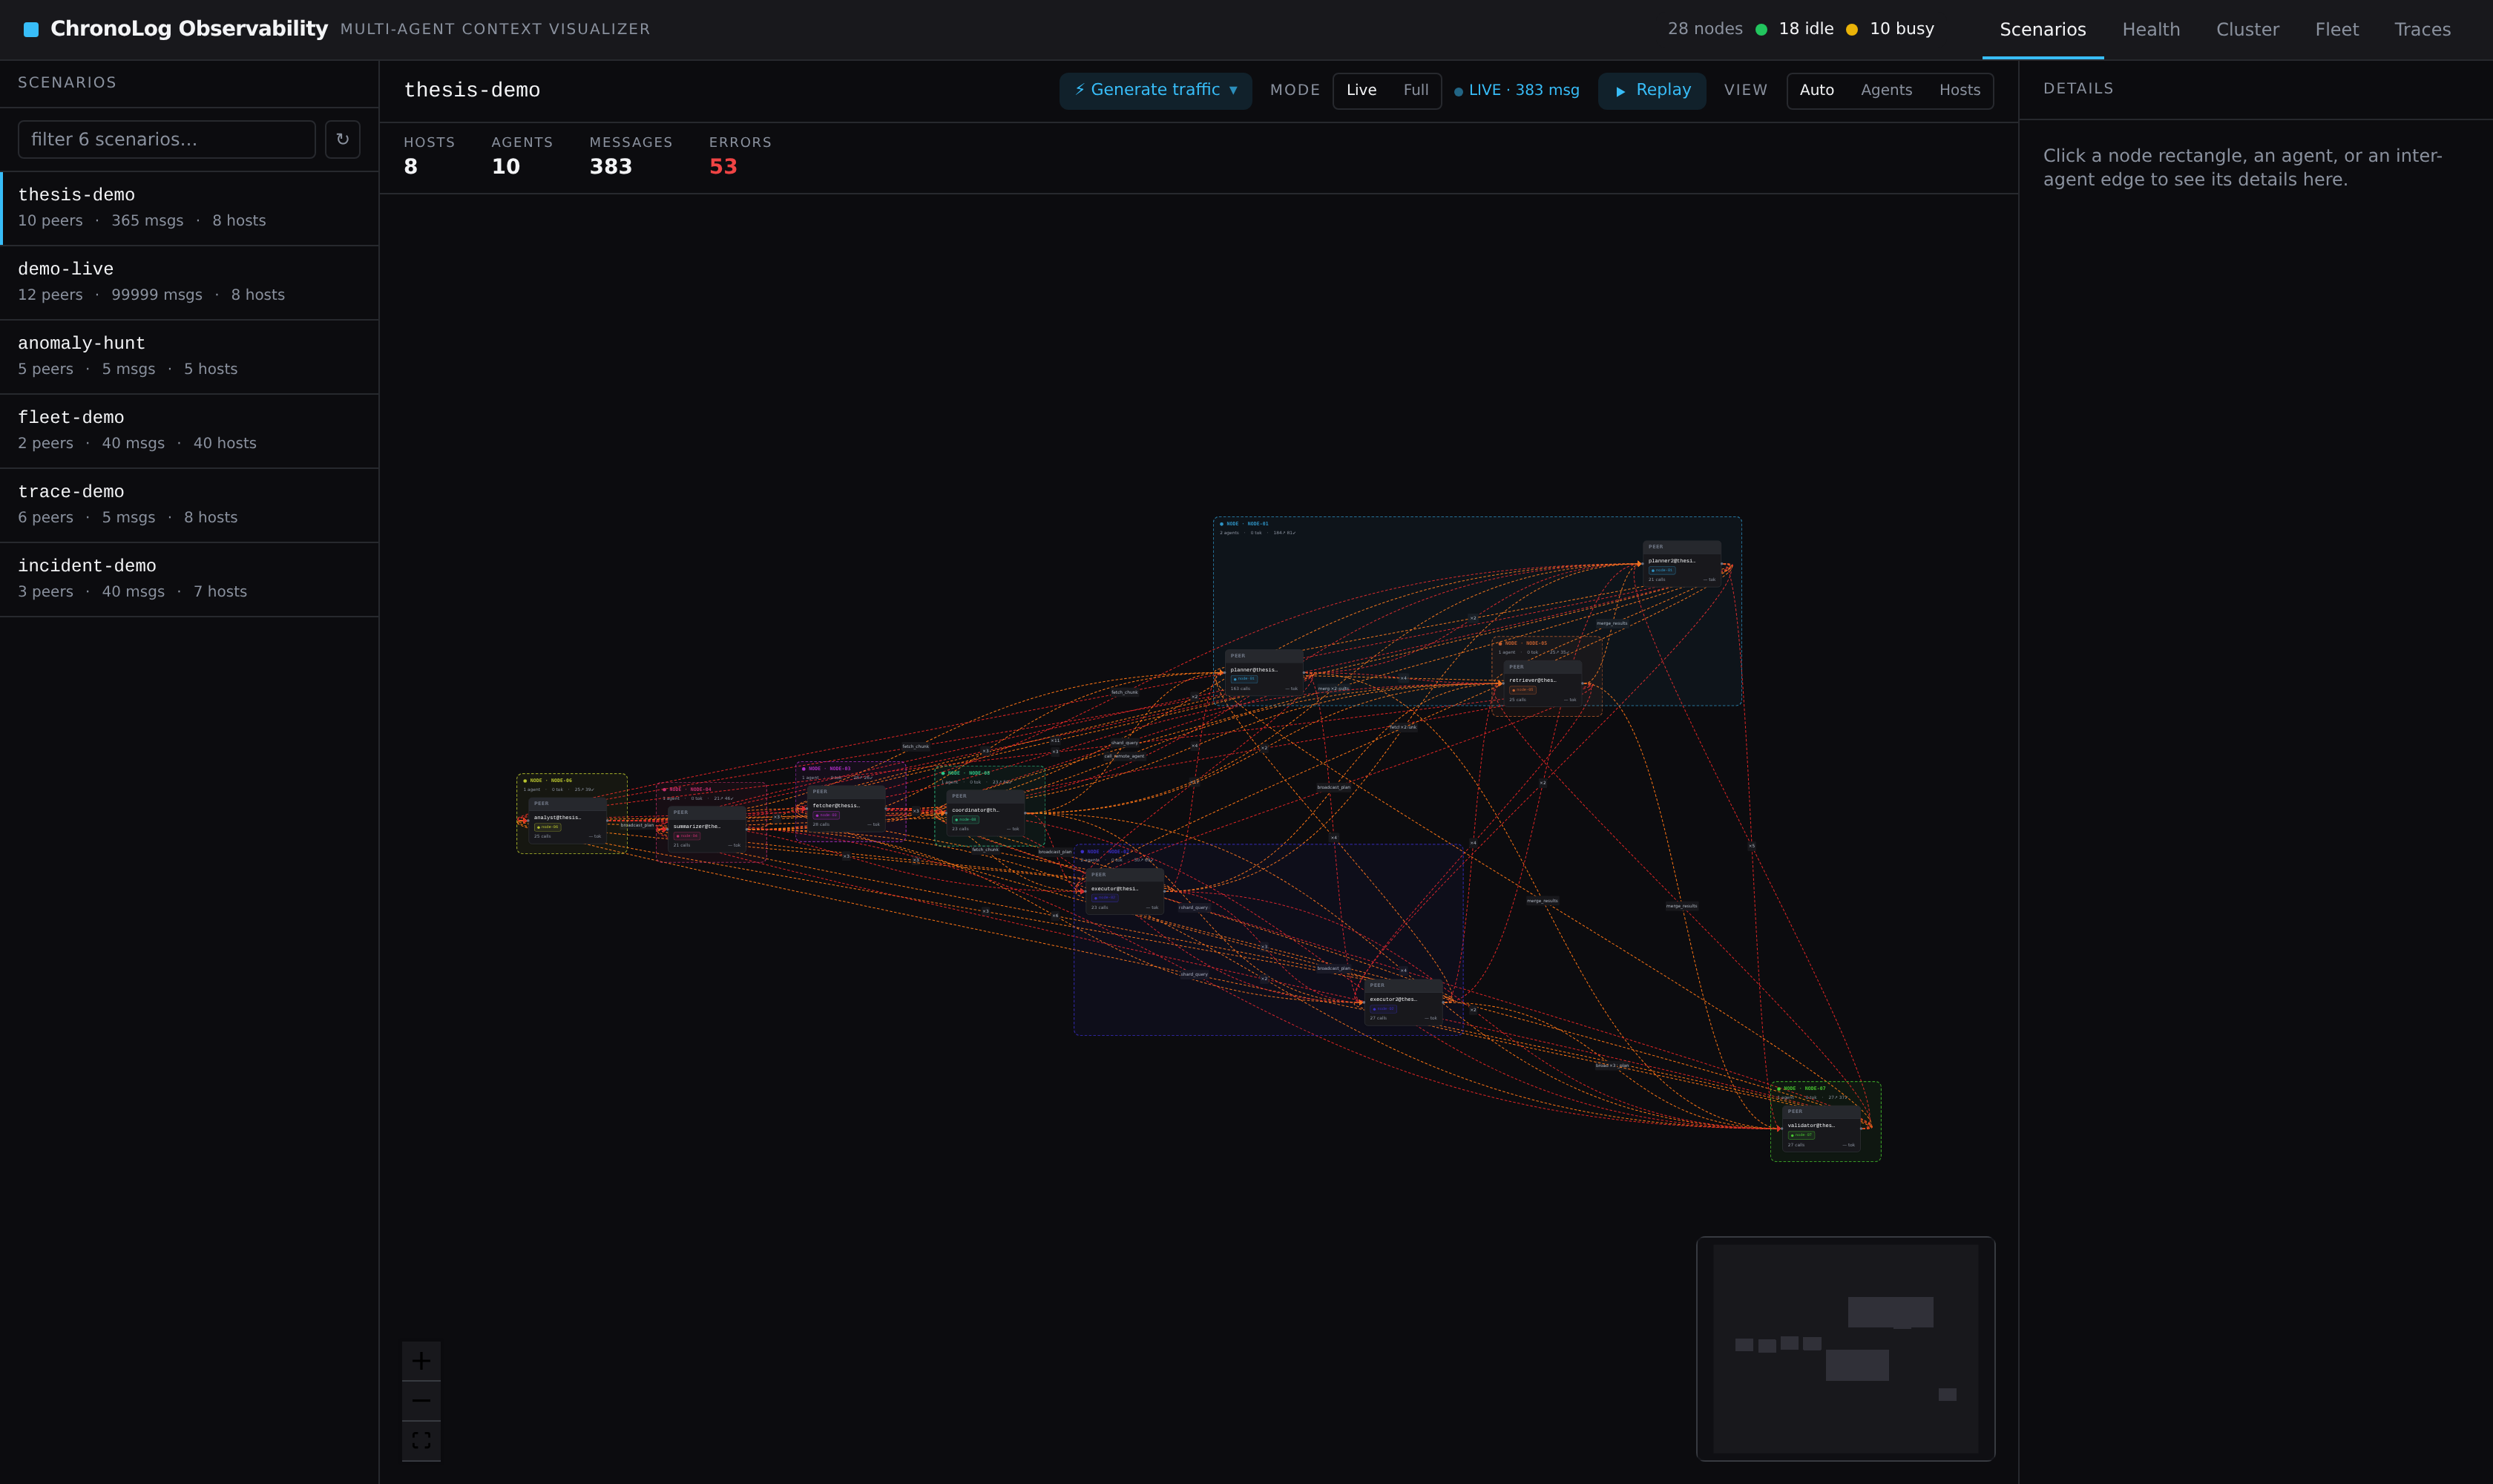
\includegraphics[width=\linewidth]{figures/ui-scenarios}
  \caption{The Scenarios view, live: 10 agents across 8 host groups,
  every inter-agent call an edge (errors red), with live message and
  error counters. Clicking a node opens the agent's conversation,
  the capture-to-conversation join of R1.}
  \label{fig:ui-scenarios}
\end{figure}

\paragraph{Health: what is wrong, and why
(Fig.~\ref{fig:ui-health}).} The ChronoDoctor surface. The center
column is the live LLM-call feed (every turn as it happens, filterable
to errors or a provider); the left rail is the ranked incident list a
scan produces: one card per clustered incident, ordered by severity,
with occurrence counts and \emph{recurring} badges read back from the
incident memory. Selecting an incident opens its diagnosis card:
\emph{why this is happening} and \emph{how to fix it} in prose, the
blast radius (occurrences, hosts, agents, scenarios), the heuristic's
stated confidence, and the raw evidence samples that justify it.
The compression argument of \S\ref{sec:analytics-doctor} is legible in
the ratio: thousands of raw signals arrive as a dozen ranked cards, each
carrying its own justification.

\begin{figure}[p]
  \centering
  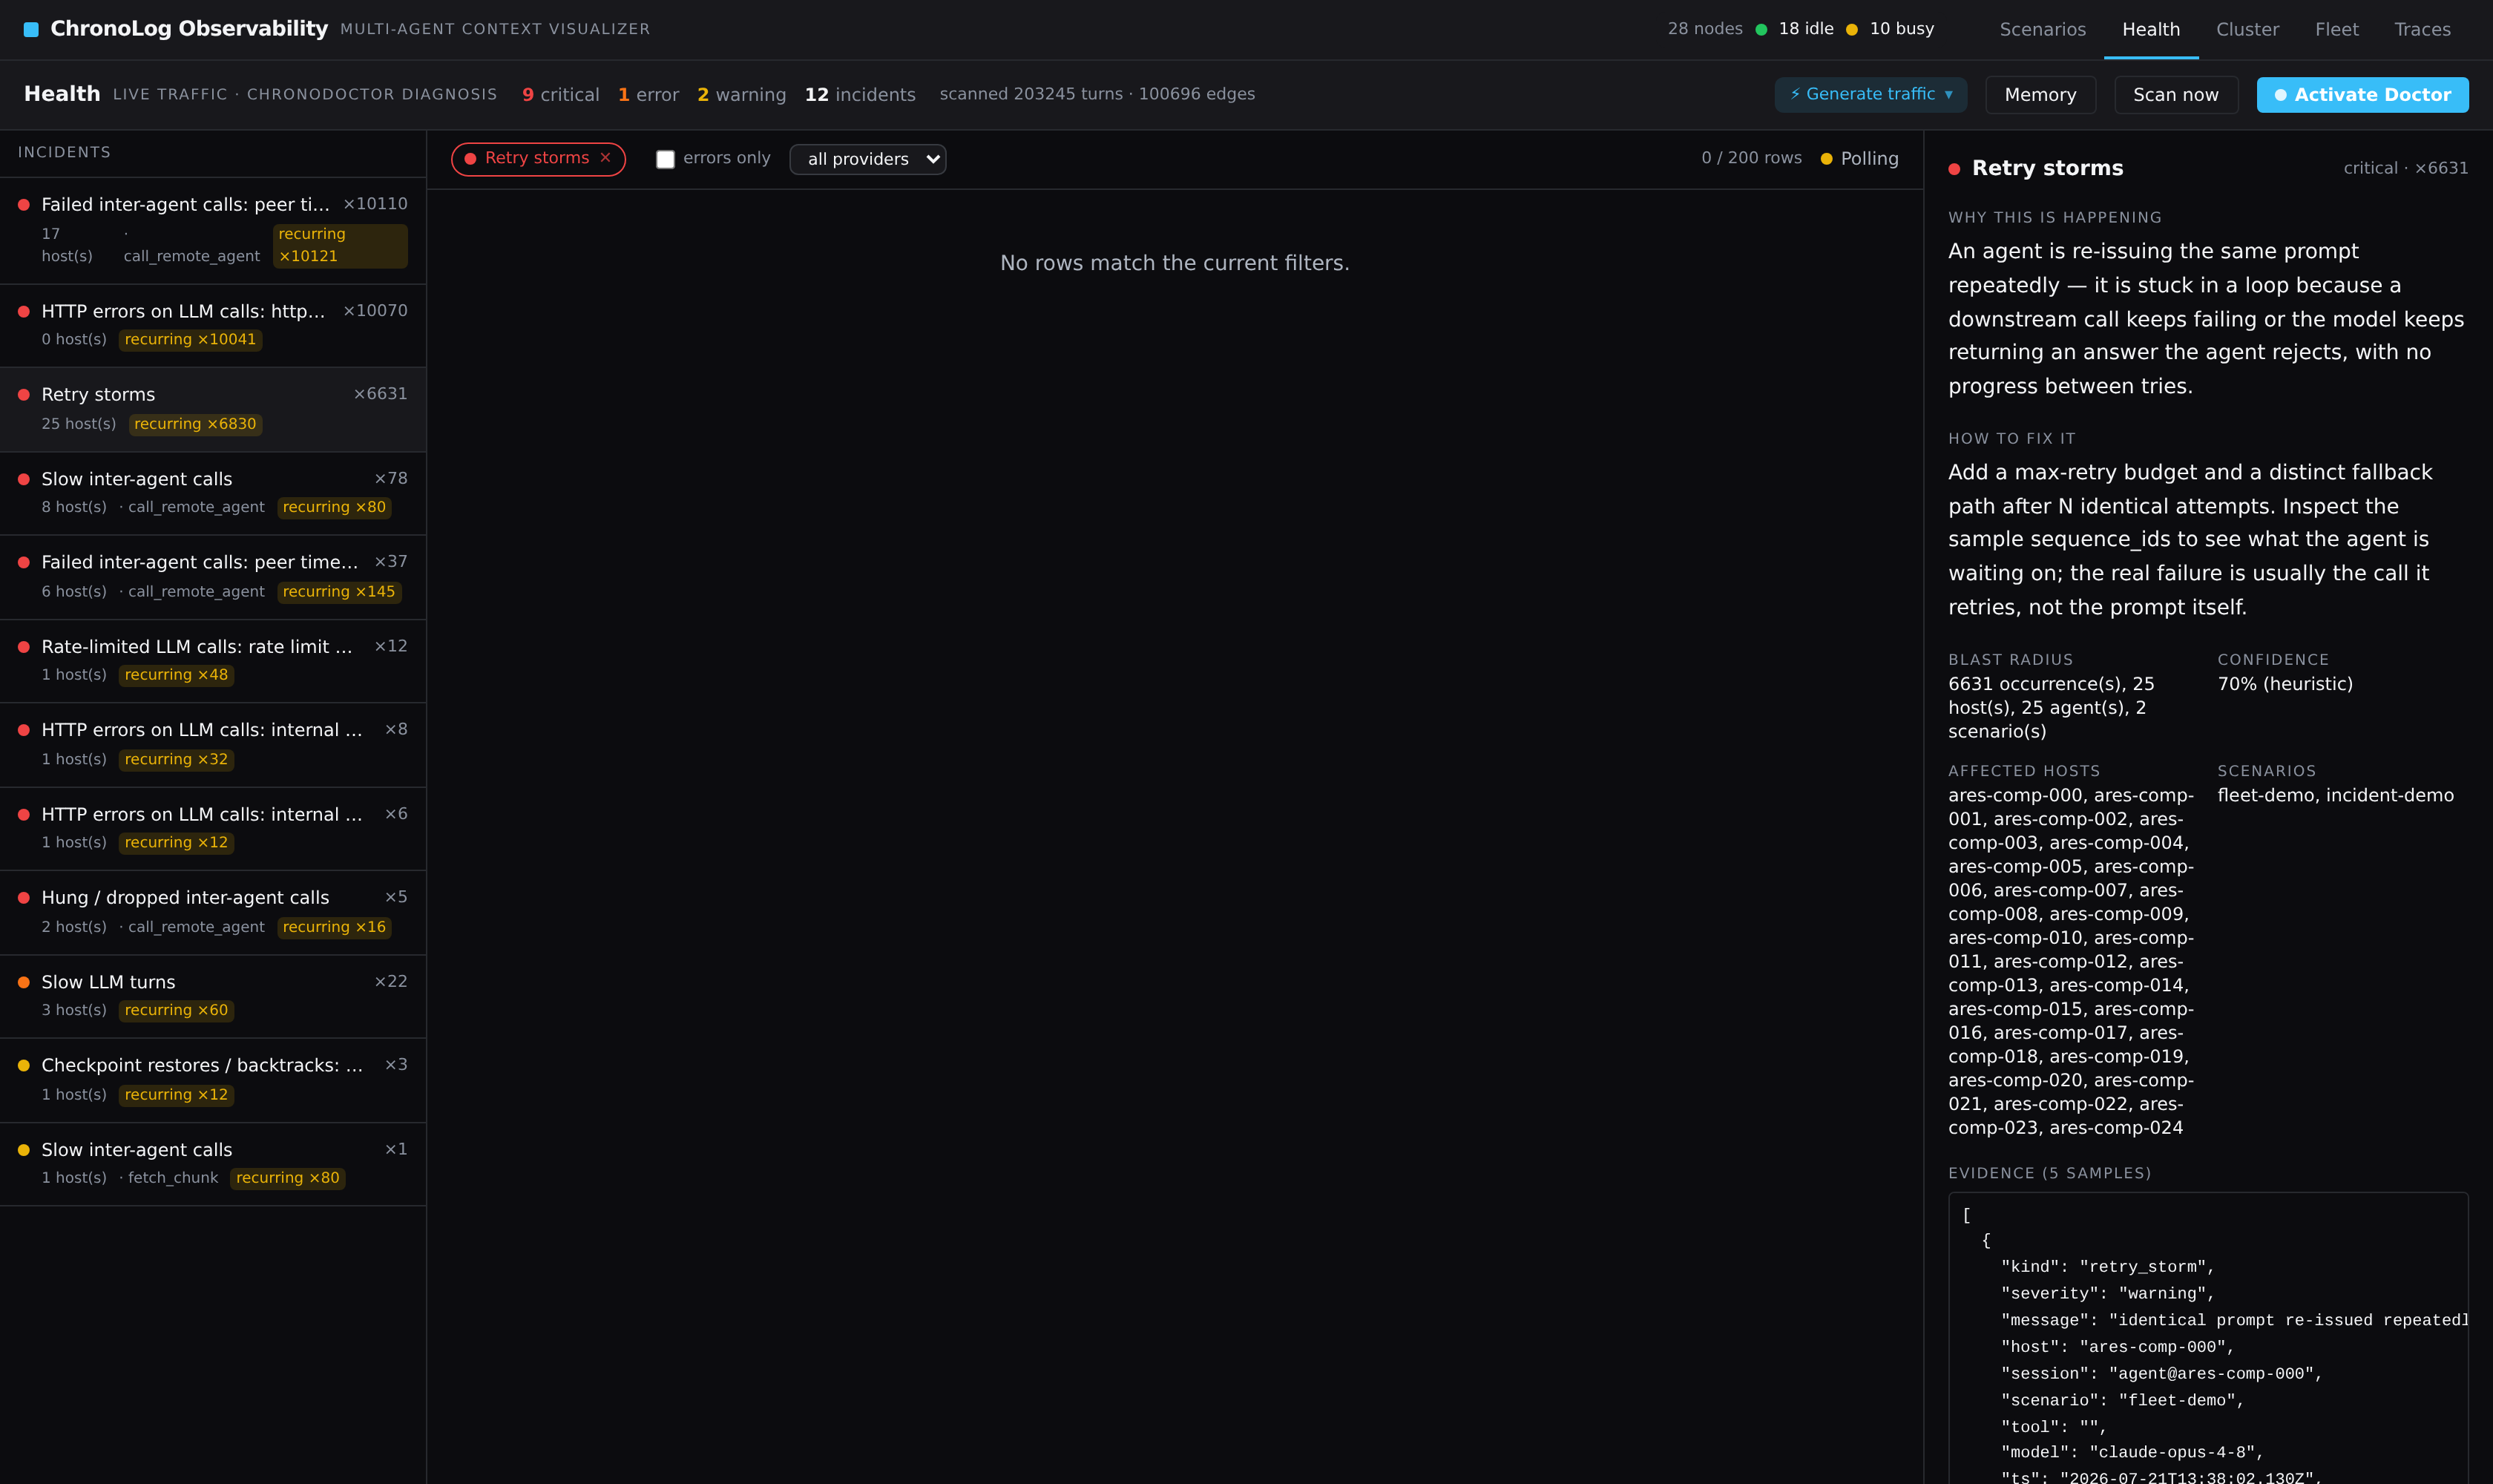
\includegraphics[width=\linewidth]{figures/ui-health}
  \caption{The Health view after a Doctor scan over a large demo
  corpus: 12 ranked incidents from ${\sim}200$\,k scanned turns (left),
  and the selected incident's diagnosis card (right) carrying root cause,
  remediation, blast radius, confidence, and evidence samples.
  \emph{Recurring} badges are read from the cross-run incident memory.}
  \label{fig:ui-health}
\end{figure}

\paragraph{Cluster: agent semantics on physical topology
(Fig.~\ref{fig:ui-cluster}).} This view puts the substrate itself on
screen: the ChronoLog
deployment drawn on the allocation's nodes (visor, one keeper
card per node with the chronicles and stories it holds, grapher and
player placement), overlaid with the cluster graph of
\S\ref{sec:analytics-topology} so that
agent traffic is visible \emph{on} the machines that carry it, next to
the SLURM capacity badge (idle/busy/down). R7 reads directly off the
picture: the same physical node hosts both an agent's runtime and
the keeper that captures it, and the operator sees both roles at once.

\begin{figure}[p]
  \centering
  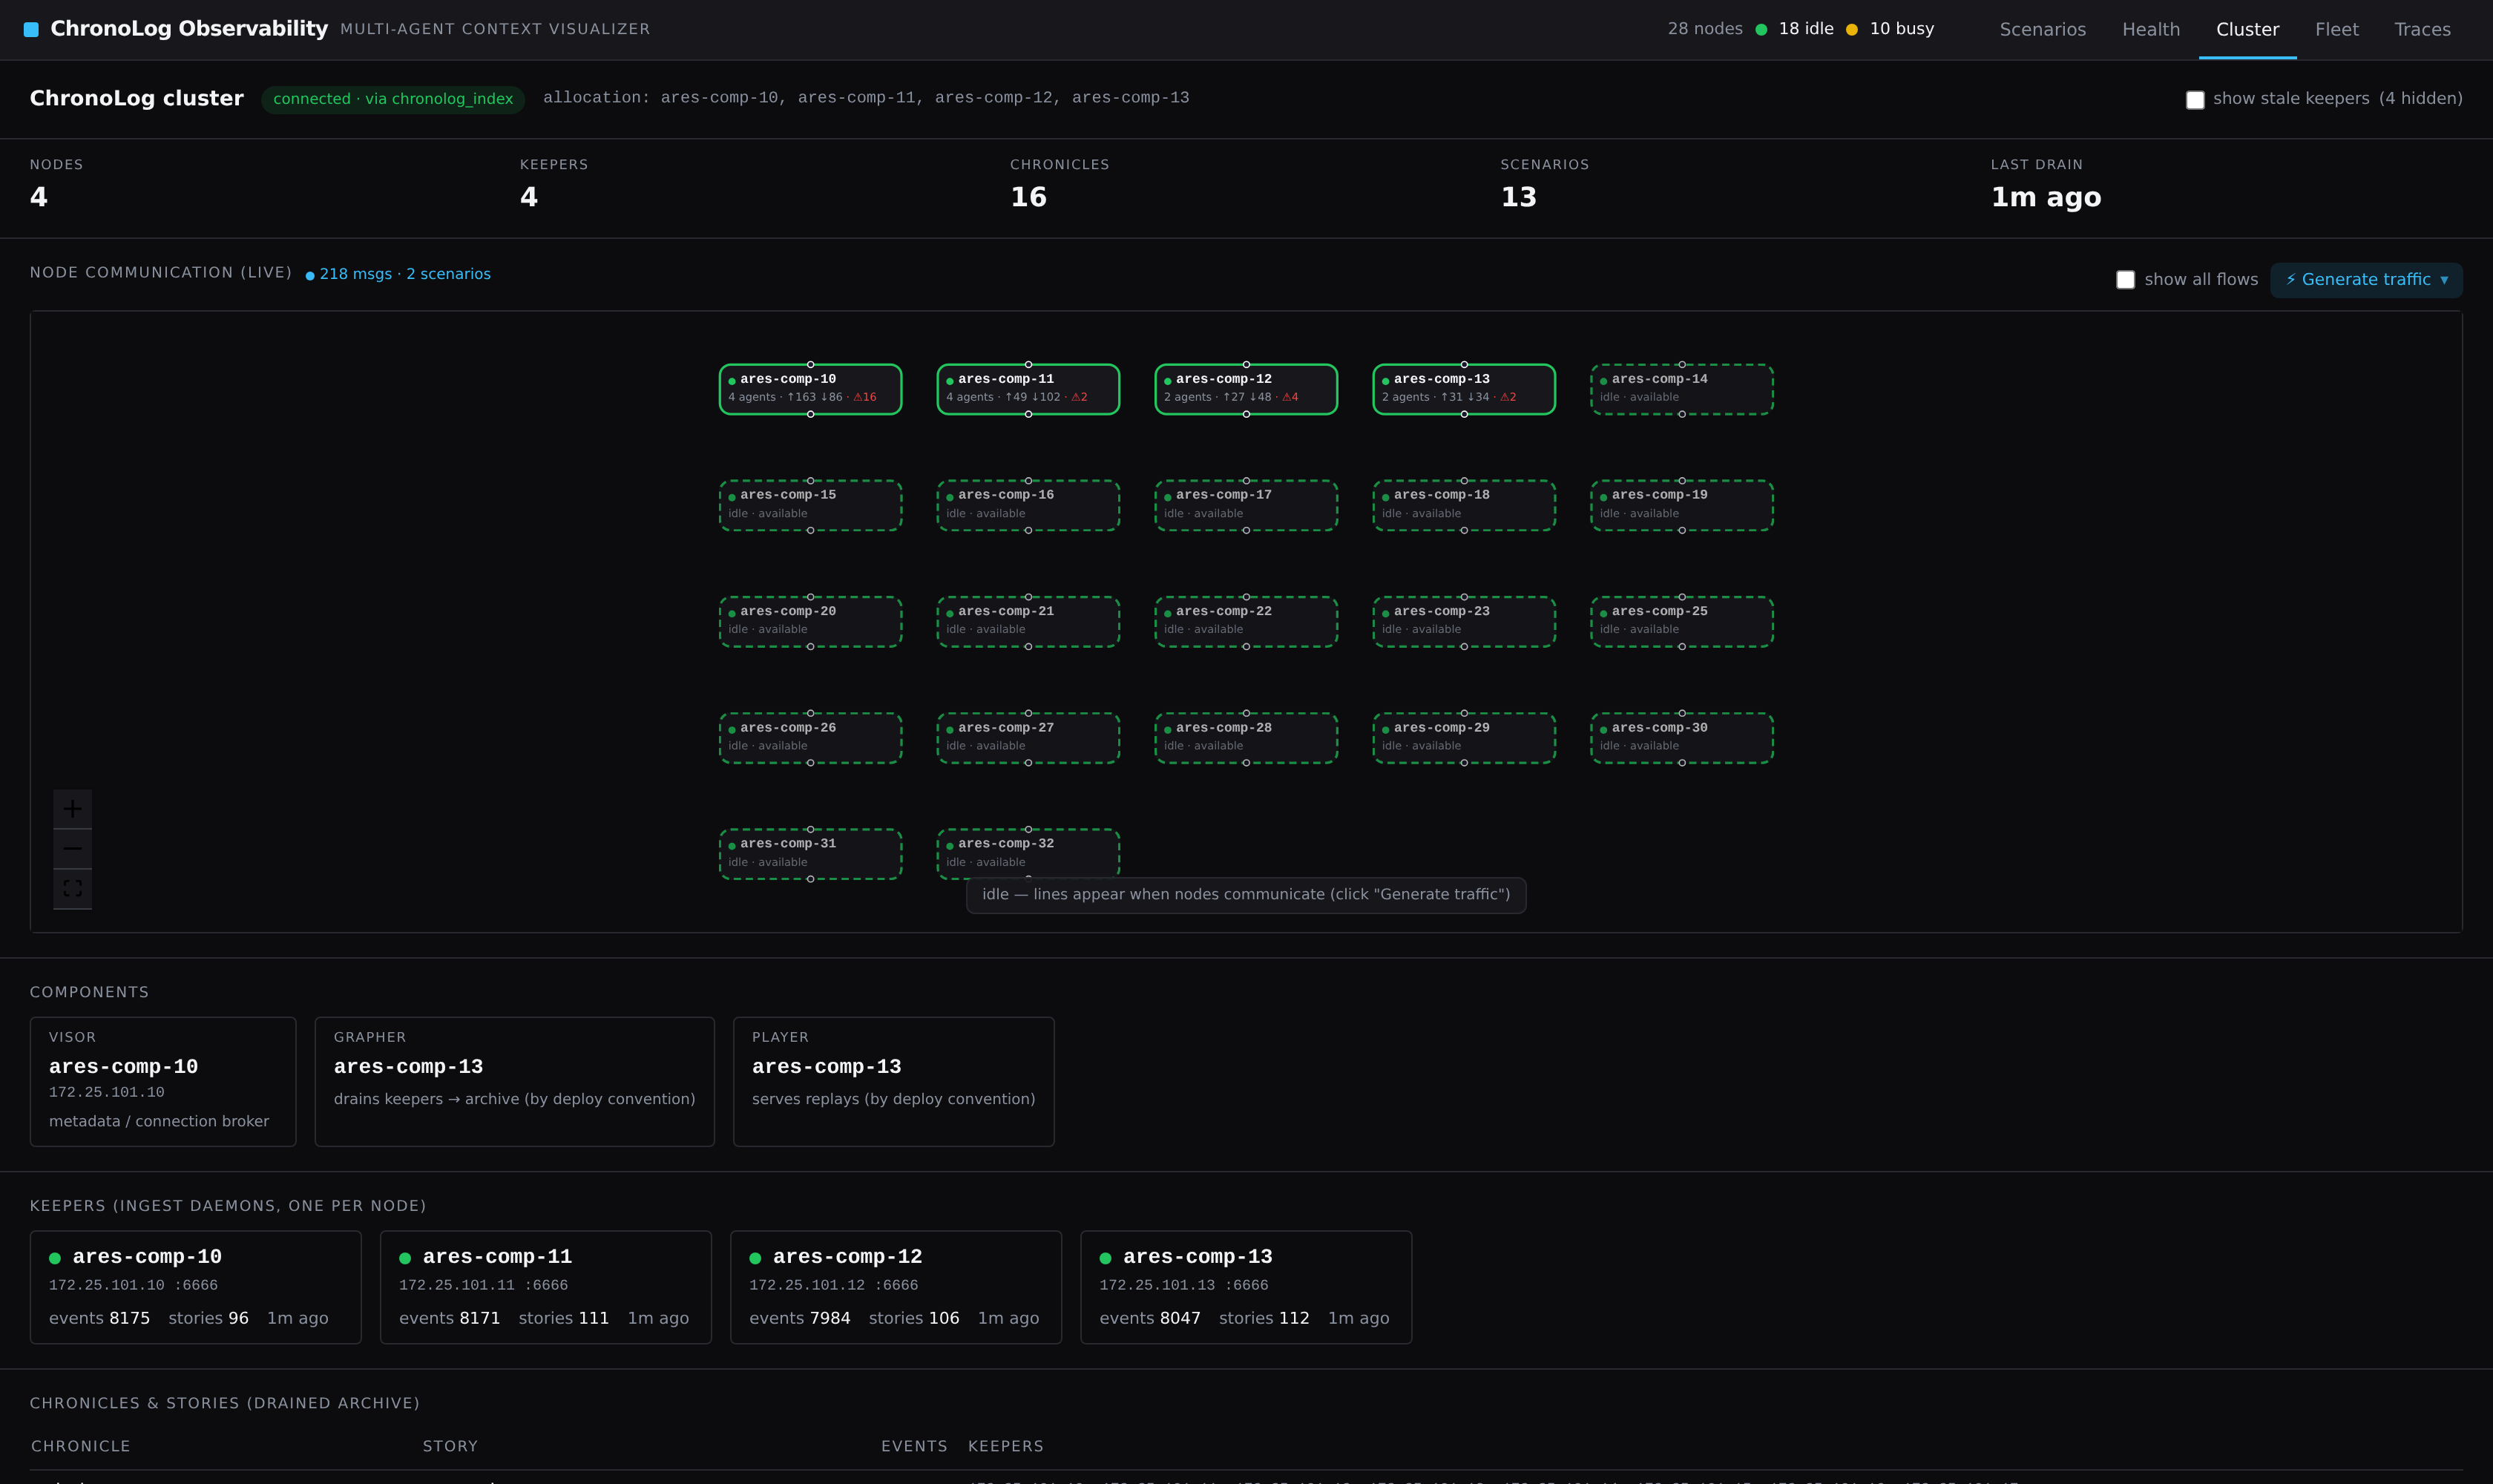
\includegraphics[width=\linewidth]{figures/ui-cluster}
  \caption{The Cluster view on a live 4-node deployment: ChronoLog
  components (visor, grapher, player placement; one keeper card per
  node with its event and story counts and last-drain age) alongside
  the live cluster graph and SLURM capacity. The headline
  freshness stat reports the \emph{measured} last-drain age
  (\S\ref{sec:eval-freshness}); the grapher's configured 180\,s
  acceptance window is relegated to its tooltip.}
  \label{fig:ui-cluster}
\end{figure}

\paragraph{Fleet: the population at a glance
(Fig.~\ref{fig:ui-fleet}).} One cell per node, colored by rolled-up
health state (ok / warn / crit, idle and busy dimmed), worst first;
the header aggregates events, errors, and cost over the selected
window. The representation change argued in
\S\ref{sec:analytics-fleet} pays off here: where the node-link graph saturates at a
dozen nodes, the heatmap stays legible at hundreds (the capture
below shows 256), and the red cells are the Q4 answer before a single
query is typed. Clicking a cell filters the fleet to that node and
hands off to the other views for the why.

\begin{figure}[p]
  \centering
  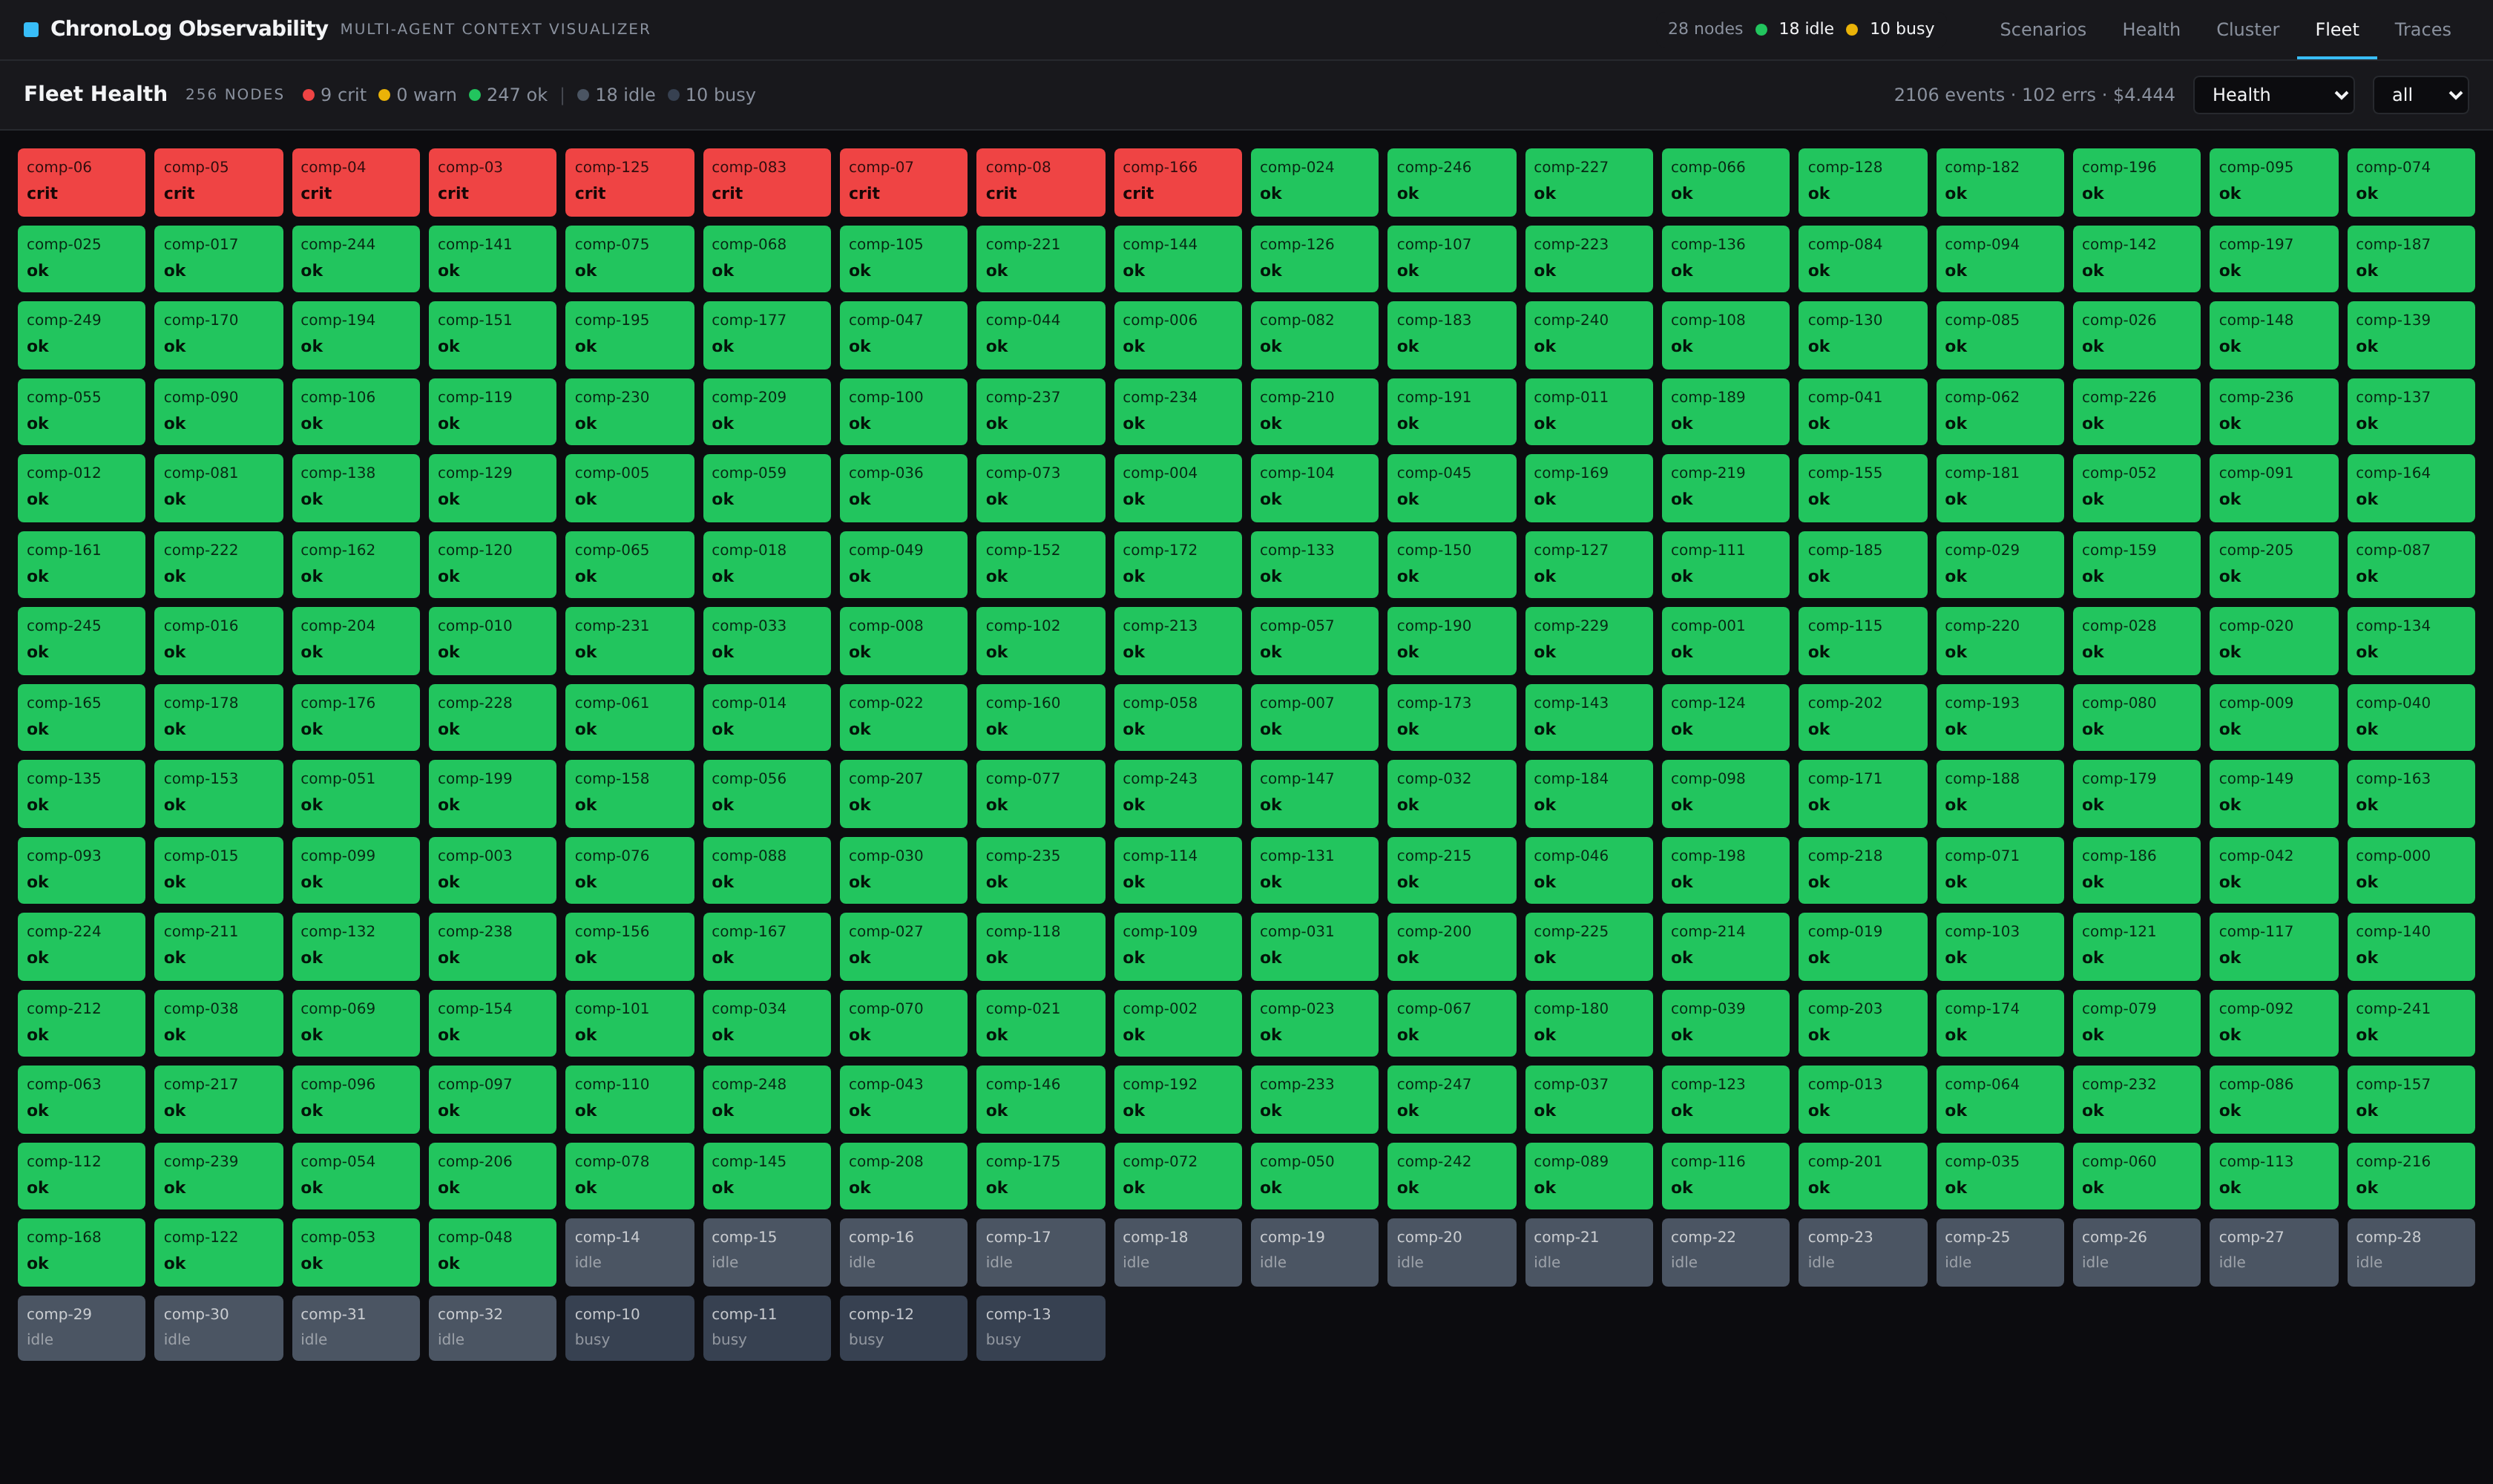
\includegraphics[width=\linewidth]{figures/ui-fleet}
  \caption{The Fleet view: 256 nodes, one cell each, rolled-up health
  worst-first. Nine critical nodes are the immediate Q4 answer.
  Rollup-backed reads keep this view interactive independent of event
  volume (\S\ref{sec:eval-scalability}).}
  \label{fig:ui-fleet}
\end{figure}

\paragraph{Traces: where the time went
(Fig.~\ref{fig:ui-traces}).} The critical-path surface of
\S\ref{sec:analytics-tracing}: traces listed slowest-first; the
selected trace rendered as a depth-indented waterfall with the critical
path outlined and each hop labeled \emph{tool $\to$ host}; the header
names the bottleneck hop with its self-time: in the capture,
\texttt{call\_remote\_agent} $\to$ \texttt{comp-04} at 12.0\,s of a
21.6\,s trace. A self-time bar above the waterfall shows at a glance
which host consumed the wall-clock, and clicking any span opens the
edge's detail. This is Q3 answered as a sentence, not a scroll.

\begin{figure}[p]
  \centering
  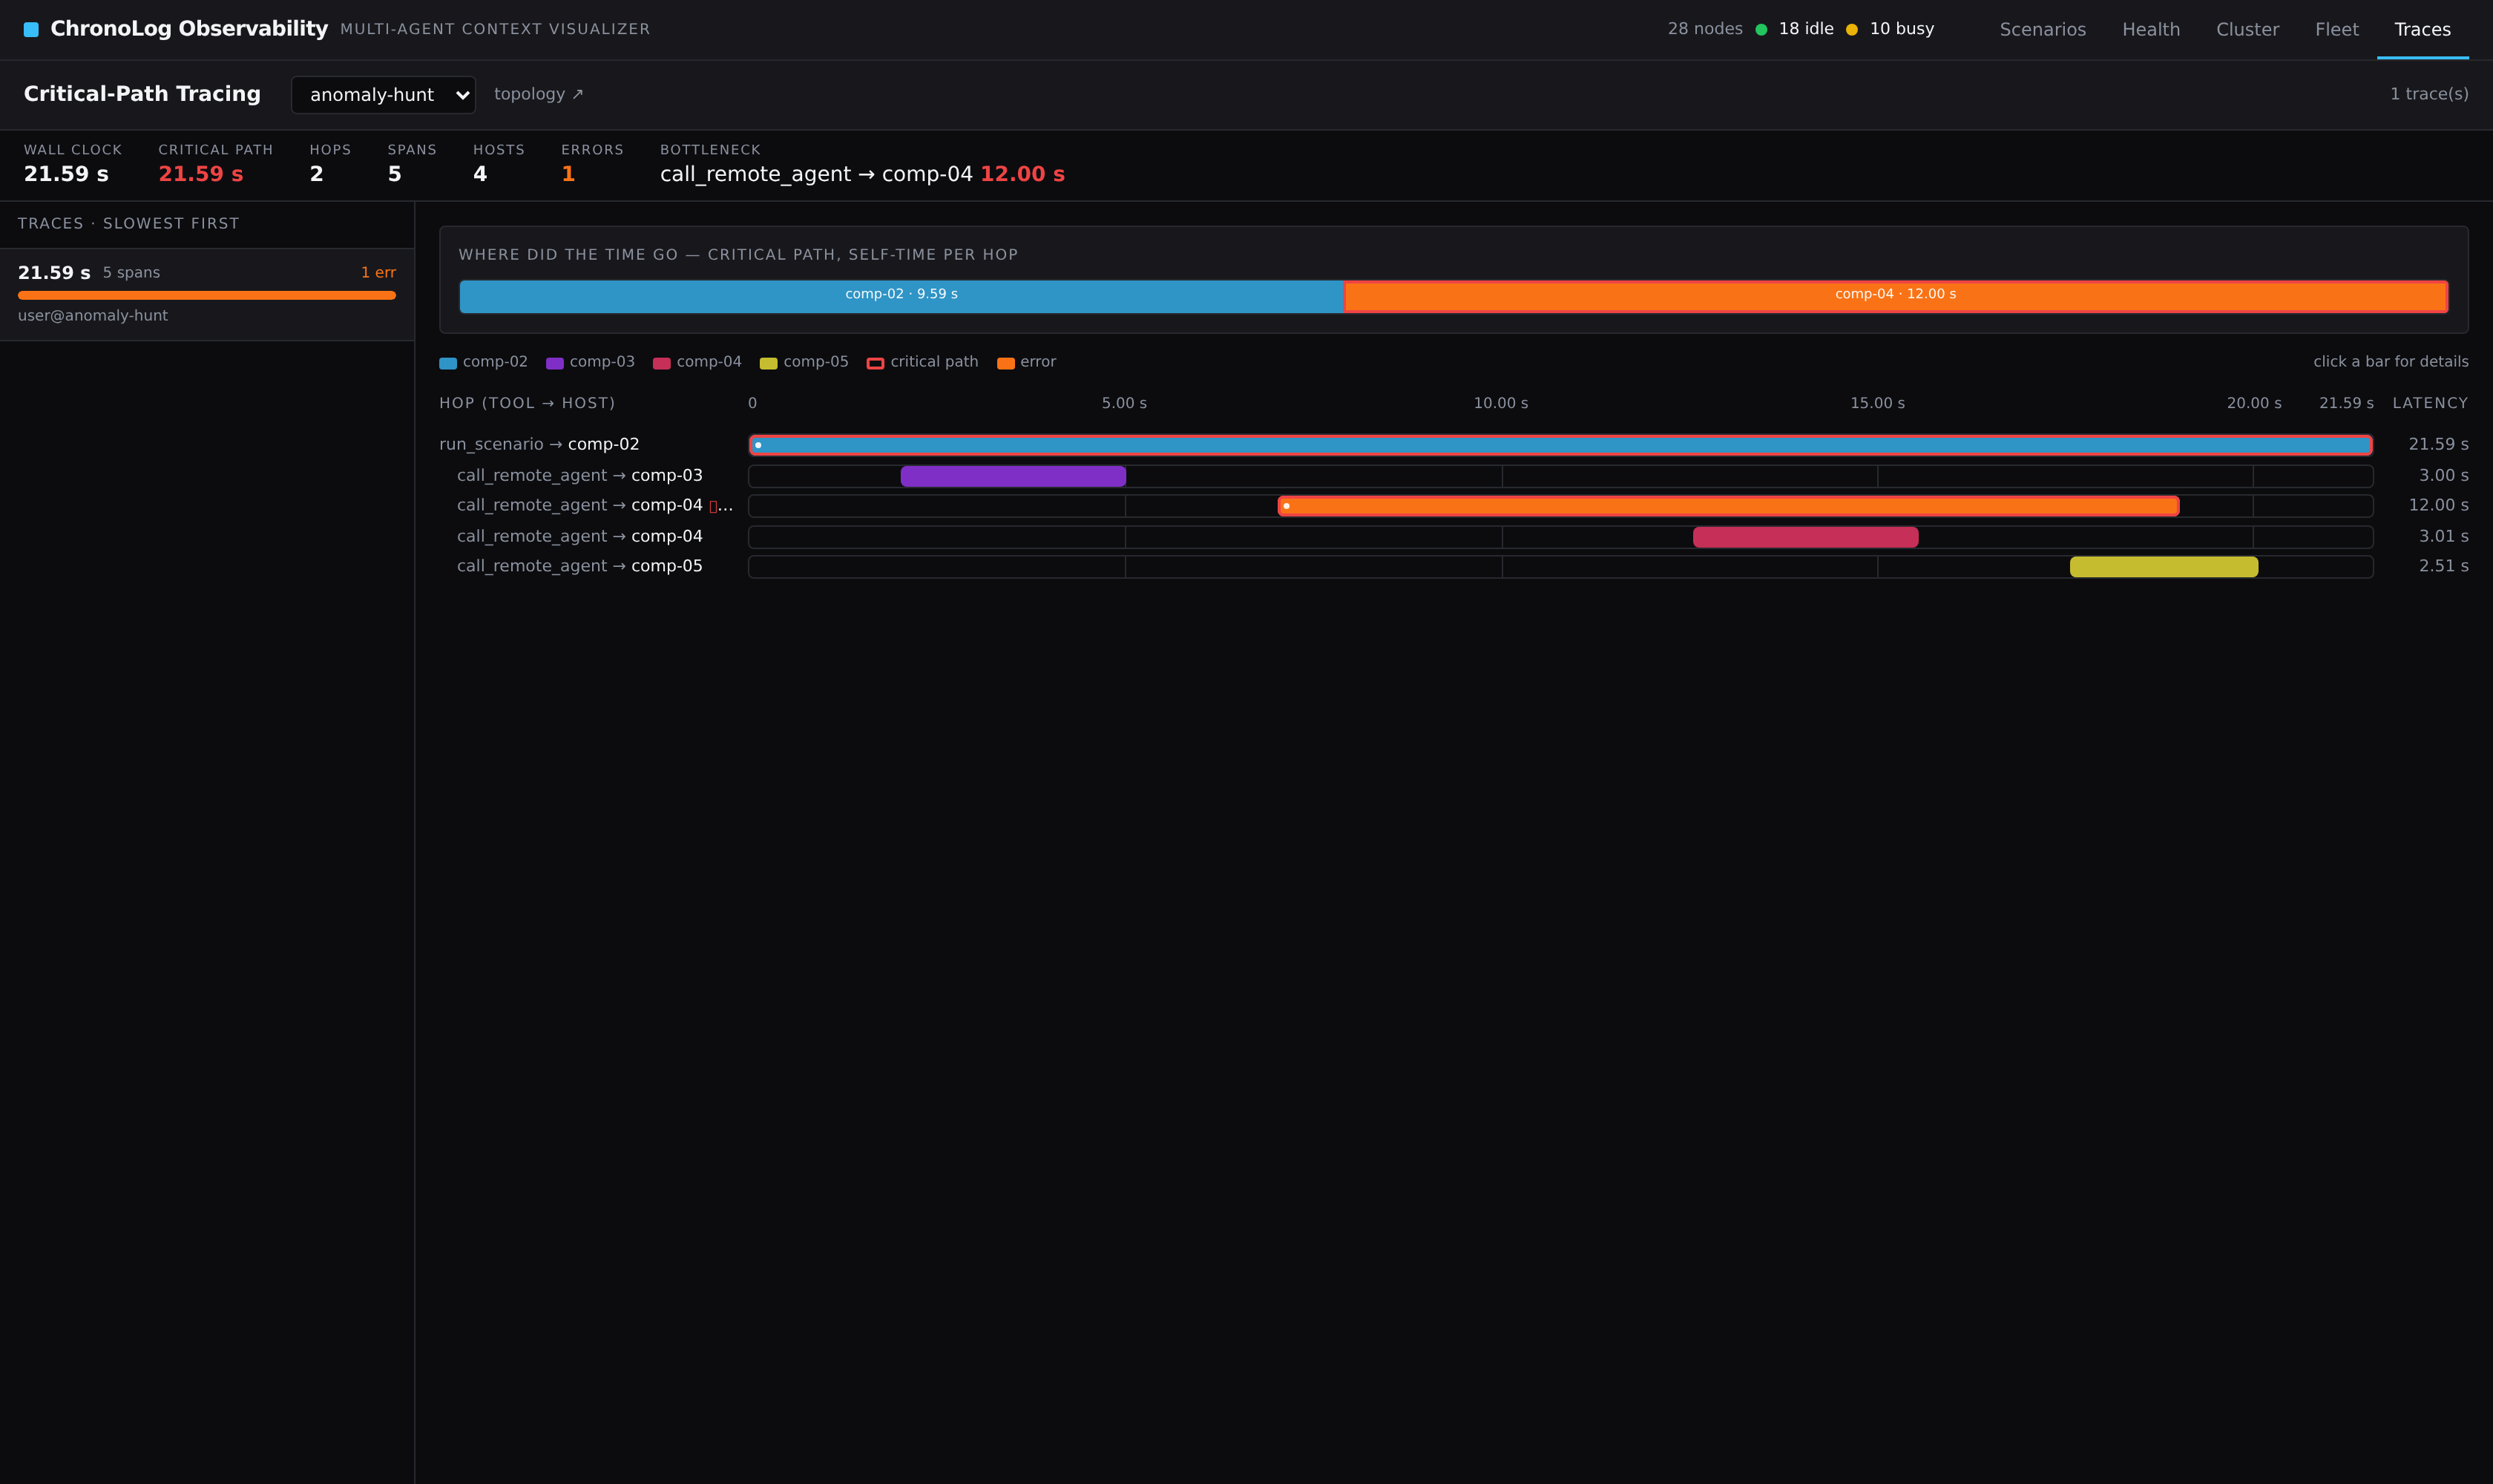
\includegraphics[width=\linewidth]{figures/ui-traces}
  \caption{The Traces view: critical-path waterfall for the slowest
  trace of a scenario. The header names the bottleneck (the
  \texttt{comp-04} hop, 12.0\,s self-time of 21.6\,s wall-clock); the
  top bar shows self-time per hop along the critical path.}
  \label{fig:ui-traces}
\end{figure}

Together the five views implement the pivot the case study of
\S\ref{sec:eval-casestudy} times end-to-end: Fleet says \emph{which
machine}, Health says \emph{what and why}, Traces says \emph{where the
time went}, Scenarios says \emph{who}, and the conversation view says
\emph{show me}. All are projections of one shared log, reachable from
each other in a click or two.
